% \begin{multicols}{2}

\section{Einleitung}

\subsection{Ziel der Arbeit}

Es soll in erster Linie ein Computer-Modell entwickelt werden, welches aufgrund eines Höhenmodells eine möglichst defensive (risikominibierende) Aufstiegsroute plant. Als Erweiterung wird dieses Modell mit einer ansprechenden 3D-Karte als Hintergrundebene in einer Webapp zur Verfügung gestellt. Die vom Modell produzierten Touren werden mit Literaturrouten aus dem Tourenportal des SAC, bzw.\ aus diversen dort gesammelten Tourenführern verglichen und ihre Begehbarkeit kritisch überprüft.

\subsection{Bestehende Referenzsysteme}

Mit dem Algorithmus von Andreas Eisenhut besteht seit 2013 eine mehr oder wenig fertig implementierte Lösung um Skitouren im Gelände automatisch zu planen\ \cite{eisenhuttourknopfdruck}. Trotz der starken Abhängigkeit von kostenpflichtigen Werkzeugen stellt diese Arbeit eine Pionierleistung in diesem Gebiet dar und wurde ebenfalls durch die Platform Skitourenguru aufgegriffen. Hier ist es jedoch nutzerseitig nicht möglich, einen Punkt A und B einzugeben und eine Route zurück zu erhalten. Zum Verfassungszeitpunkt dieser Arbeit kann die öffentlich zugängliche Version des Tools nur verwendet werden um bestehende GPS-Tracks und von Hand gezeichnete Routen idealer zu legen. Die Thesis von A. Eisenhut wurde wären dem Implementationsprozess dieser Arbeit nicht referenziert, erst während dem Verfassen der finalen Arbeit.

\section{Grundlagen der Lawinenkunde}
\subsection{Analytische vs. Praktische Lawinenkunde}
Lawinenprobleme lassen sich grundsätzlich aus zwei Perspektiven betrachten und vorhersagen: Einerseits auf Basis der Schneedecke, anderer seits auf Basis von Geländeformen und Statistik.
Dabei wird bei der praktischen Lawinenkunde auf das erstellen von beispielsweise Schneeprofilen (Extended Coloumn Test) zur Einschätzung der lokalen Stabilität der Schneedecke gesetzt.

Bei der analytischen Lawinenkunde arbeiten wir mit historischen Unfalldaten, konkret ist das Ziel, ein quantitatives Mass für das eingegangene Risiko zu errechnen.
Daraus leiten wir die Entscheidung ab, weiter aufzusteigen oder umzukehren – diese Entscheidung steht in beiden Gebieten im Vordergrund.

\subsection{Lawinentypen}

Lawinen lassen sich anhand ihrer Auslösemechanismen, des Materials, das sie transportieren, und der spezifischen Bedingungen, unter denen sie entstehen, klassifizieren. Die wichtigsten Lawinentypen --- Schneebrettlawinen, Lockerschneelawinen, Gleitschneelawinen (und Staublawinen) --- unterscheiden sich in ihrer Entstehung, Dynamik und den daraus resultierenden Gefahren. Eine genaue Kenntnis dieser Unterschiede ist notwendig für die Lawinenkunde und das alpine Risikomanagement.

%TODO: Seitenumbrüche hier prüfen

\begin{enumerate}
  \item Schneebrettlawinen~\cite{sacbergspwinter}\cite{slfLawinentypen}:
  \begin{itemize}
    \item Fordern 90\% der Lawinenopfer
    \item Abriss entlang einer Kante, Schnee gleitet als ganzer Block <<Brett>> ab
    \item Brett gleitet auf einer darunterliegenden Schwachschicht in der Schneedecke ab
    \item Kann aufgrund von Mehrbelastung durch Wintersportler oder spontan abgehen
    \item Auslösender Athlet steht oft mitten im Schneebrett
    \item Verschüttungsgefahr gross –\\ Mitreis- \& Absturzgefahr gross
    \item Gefahr ab einer Hangneigung von $30\degree$
  \end{itemize}
  % % \columnbreak{}
    
  \item Lockerschneelawinen~\cite{sacbergspwinter}\cite{slfLawinentypen}:
  \begin{itemize}
    \item Punktförmiger Auslösepunkt
    \item Reisst immer mehr Schnee mit, Kegelförmiger Abgang der nach unten breiter wird
    \item Verschüttungsgefahr klein –\\ Mitreis- \& Absturzgefahr gross
    \item Im Auslösepunkt ist meistens eine hohe Steigung von $40\degree$ notwendig
  \end{itemize}

  \item Gleitschneelawinen~\cite{sacbergspwinter}\cite{slfLawinentypen}:
  \begin{itemize}
    \item Ebenfalls linienförmige Abrisskante
    \item Die gesamte Schneedecke gleitet ab
    \item Kleine Bedeutung für Wintersportler –-- gehen oft spontan ab und gefährden vor allem Infrastruktur (Abgleiten erfolgt über mehrere Stunden oder Tage hinweg, zeigt sich gut durch sog. <<Fischmäuler>>)
  \end{itemize}
\end{enumerate}
Für unsere Zwecke interessieren uns an erster Stelle \textbf{Schneebrettlawinen} und an zweiter \textbf{Lockerschneelawinen}, da diese Lawinentypen für die meissten Unfälle mit Personenschaden abseits der Schweizer Pisten verantwortlich sind. In $\qty{95}{\percent}$ aller Unfälle lösen Schneesportler dabei ihre Unglückslawine selbst aus~\cite{ortovoxlabsnow}. Aus diesem Grund wird im weiteren Verlauf dieser Arbeit einer möglichen Fernauslösung keine weitere Beachtung geschenkt.

% \pagebreak
\subsection{Typische Lawinenprobleme}\label{lawinenprobleme}

In der Lawinenkunde werden bestimmte Lawinenprobleme definiert, um die komplexen Zusammenhänge einfacher verständlich zu machen und die Risikoanalyse zu erleichtern. Diese typischen Lawinenprobleme umfassen verschiedene Szenarien, die besonders häufig auftreten und die Lawinengefahr massgeblich beeinflussen. Ein tiefes Verständnis dieser Probleme ist von Nöten, um in gefährdetem Gelände sicher unterwegs zu sein und präzise Entscheidungen in Bezug auf Lawinensicherheit zu treffen.

\begin{enumerate}
  \item Neuschneeproblem~\cite{achtunglawine}:
  \begin{itemize}
    \item Frischer Neuschnee, welcher sich schlecht mit der darunterliegenden Schneeschichten verbunden hat. 
    \item Produziert ab der kritischen Neuschneemenge (je nach Bedingungen zwischen \qty{10}{cm} --~\qty{50}{cm}) mindestens die Warnstufe <<3 -~Erheblich>> im \acrfull{llb}.\@
    \item Setzt sich in 2 bis 3 Tagen
  \end{itemize}
  \item Triebschneeproblem~\cite{achtunglawine}:
  \begin{itemize}
    \item Wind trägt Neuschnee in Windschattenlagen
    \item Triebschnee verbindet sich leicht mit sich selbst, jedoch nicht mit darunterliegenden Schichten; ideale Voraussetzungen für ein Schneebrett
    \item Gefahr durch Schneeverfrachtungen (z.B. auch Wechten)
    \item Setzt sich innert 2 bis 3 Tagen
  \end{itemize}
  \item Nassschneeproblem~\cite{achtunglawine}:
  \begin{itemize}
    \item Die Schneedecke wird durch eindringendes Wasser geschwächt
    \item Die erste Durchfeuchtung führt zu der bedeutendsten Schwächung
    \item Gefahr nach andauernden Regenperioden im Winter
    \item Typische Frühlingslawinen, steigende Gefahr im Verlauf des Tages mit steigender Temperatur
    \item Lange anhaltende Gefahr
  \end{itemize}
  \item Altschneeproblem~\cite{achtunglawine}:
  \begin{itemize}
    \item z.B. Eingeschneite Harschschichten schwächen die Schneedecke erheblich
    \item Dauert Wochen bis Monate an
  \end{itemize}
\end{enumerate}
Es ist möglich, das mehrere Lawinenproblem miteinander auftreten. Im \gls{llb} sind jeweils alle zu erwartenden Lawinenprobleme mit einer eigenen Gefahrenstufe aufgeführt.~\cite{slfTypischeLawinenprobleme}

\subsection{Lawinenlagebericht (Bulletin) \& Gefahrenstufen}

Im Lawinenbulletin/Lawinenlagebericht, kurz \gls{llb}, werden die momentan am Berg zu erwartenden Lawinenprobleme (siehe~\ref{lawinenprobleme}) zusammengefasst und mit diversen zusätzlichen Datenprodukten ergänzt.

Abb.\ \ref{fig:bulletin} zeigt ein Beispiel eines \gls{llb} Bulletins, wie dieses während dem Winter täglich erscheint.

In der europäischen Lawinengefahrenskala werden fünf Warnstufen unterschieden, von <<1 -~gering>> bis <<5 -~sehr gross>>.~\cite{lawinengefskala} 
Rund 50\% der Unfälle geschehen dabei bei <<3~-~mässig>>~\cite{achtunglawine}.

\begin{figure}[H]
  \centering
  \includegraphics[width=7.5cm]{bulletin}
  \caption{Bulletin vom 12.2.24~\cite{slfarchiv}}\label{fig:bulletin}
\end{figure}

Die Skala ist kontinuierlich, jedoch nicht linear. Heisst konkret: 
Im Durchschnitt ist das Risiko bei <<mässig>> fünf Mal so hoch wie bei <<gering>>, und bei <<erheblich>> drei Mal so hoch wie bei <<mässig>>~\cite{sacbergspwinter}. (Siehe Abb.\ \ref{fig:llbdanger})

\begin{figure}[H]
  \centering
  \includegraphics[width=7.5cm]{gefahrenstufen}
  \caption{Die 5 Europäsischen Lawinengefahrstufen in einem Graph}\label{fig:llbdanger}
\end{figure}

Um die Einteilung dieser fünf Kategorien weiter zu verfeinern, wurden in der Schweiz zusätzlich Teilabstufen mittels $+$, $-$ und $=$ eingeführt (So lautet die Warnstufe im Bericht nun z.B.\ $3+$, wenn die tatsächliche Gefahr bereits nahe an einer $4$ bzw.\ $4-$ liegt)~\cite{sacbergspwinter}.
unterschiedliche Interpretation der standartisierten europäischen Skala sorgen leider dafür, das Differenzen zwischen Schweizerischen und Ausländischen Vorhersagen bestehen. Dies stellt besonders in Grenzregionen ein Problem dar, in dieser Arbeit im weiteren jedoch keine Beachtung geschenkt.


\subsection{Lawinenbildende Faktoren}

Lawinen sind das Resultat eines unglücklichen Zusammenspiels drei wesentlicher Faktoren: 
\textbf{Verhältnisse} (Wetterlage und Zustand der Schneedecke), \textbf{Gelände} (Neigung, Exposition, Höhe) und \textbf{Mensch} (95\% aller Lawinen mit Personenschaden wurden durch Menschen ausgelöst)~\cite{ortovoxlabsnow}.

Weder die Verhältnissen noch das Gelände lässt sich direkt von Wintersportlern beeinflussen. Nur durch die Wahl eines anderen Datums (nur in Ausnahmefällen sinnvoll, z.B.\ bei einer Erstbesteigung), oder durch clever Spuranlage lasen sich diese Faktoren mildern. 
Ist beides keine Option, muss eine alternative Tour ausgewählt werden.
Den grössten Einfluss hat bei weitem die maximale Hangneigung --- daher konzentrieren sich die meisten gängigen Reduktionsmethoden vor allem darauf.

\subsection{Schema 3~\texttimes~3}
Der Goldstandard der Tourenplanung ist heute Werner Munters $3\times3$-Schema. Dabei werden in drei <<Zoom>>-Stufen drei Faktoren ausgewertet:
% \vfill
\textbf{Regional} 
Von zuhause aus~\cite{munter}:
\begin{itemize}
  \item Verhältnisse: 1. Lawinenlagebericht \gls{llb}, 2. Wetterprognose, 3. Auskünfte von Einheimischen/Hüttenwart
  \item Gelände: 1. $1:25000$-Karte, 2. Tourenführer, 3. Eigene Geländekentnisse
  \item Menschen: 1. Wer ist Dabei?, 2. Ausbildung, 3. Material, 4. Mentale und Phyische Kondition? 
\end{itemize}

\textbf{Lokal} Im Gebiet, auf Sichtdistanz~\cite{munter}\cite{redbull3x3}:
\begin{itemize}
  \item Verhältnisse / Schneedecke / Wetter: 1. Sicht?, 2. Bewölkung, Wind, Niederschlag, Temperatur?, 3. Schneeverfrachtungen, Neuschneemenge, 4. Stimmt der \gls{llb}?\
  \item Gelände: 1. Stimmt meine Vorstellung (Steilheit, Exposition)? 2. Spuren anderer Gruppen
  \item Menschen: 1. Ausrüstungskontrolle (Gruppencheck LVS), 2. Andere Gruppen unterwegs?
\end{itemize}
\textbf{Zonal} Im Einzelhang~\cite{munter}\cite{redbull3x3}:
\begin{itemize}
  \item Verhältnisse: 1. Neuschneemenge, 2. Triebschnee, 3. Mögliche Abrisszonen, 4. Sonneneinstrahlung
  \item Gelände: 1. Wer / was ist über/unter der Gruppe?, 2. Steilste Stelle?, 3. Exposition, 4. Typisches Lawinengelände, 5. Hangform, 6. Höhe, 7. Oft befahren?
  \item Menschen: 1. Können \& Kondition, 2. Vorischtsmassnahmen, 3. Sichere Sammelstellen
\end{itemize}

\subsection{Grafische Reduktionsmethode \& Relevante Geländefaktoren}

Die momentan am meisten verwendete Reduktionsmethode ist dabei wohl die sog.\ \gls{grm}.\@Bei dieser wird --- je nach prognostizierter Ausgeprägtheit eines Lawinenproblemes --- nur die lokale Hangneigung an einer Stelle zur Entscheidungsfindung eingesetzt~\cite{sacbergspwinter}. In der Plannungsphase wird die Hangneigung aus einer $1:25000$er-Karte mittels Neigungsmesser herausgelesen. Dies liefert jedoch nur die durchschnittliche Neigung des Geländes zwischen den Höhenlinien --- eine möglichen steileren Hangabschnitt sieht man also nicht.
Unterwegs kann entweder mittels Smartphone, Skistöcker oder Pendel die Hangneigung ermittelt werden. Es kann nun in der Grafik (siehe Abb.\ \ref{fig:grm}) herausgelesen werden, ob das zu überprüfende Gelände problemlos, nur mit Vorsichtsmassnahmen oder gar nicht betreten werden darf.

\begin{figure}[H]
  \centering
  \includegraphics[width=7.5cm]{grm}
  \caption{\gls{grm}-Karte~\cite{achtunglawine}}\label{fig:grm}
\end{figure}

An der grafische Reduktionsmethode wird oft kritisiert, dass sich zu stark auf die Hangneigung gestützt wird. Deshalb wird diese oft zusammen mit sog. <<Mustern>> gelehrt. Diese beschreiben einige Warnzeichen und wie diese das Risiko beeinflussen~\cite{achtunglawine}. Letztendlich bleibt die \gls{grm} jedoch, wie der Name verrät, eine Reduktionsmethode --- es werden selektiv die in die Auswertung einfliessenden Parameter reduziert.

\subsection{Unfalldaten \& Begehungen}

Hänge, deren steilste Stelle mindestens ca. 30° geneigt ist gelten als Lawinengefährdet. Etwa 18° geneigtes Gelände wird am häufigsten begangen, zwischen 30° und 40° Steigt das Lawinenrisiko enorm an.~\cite{sacbergspwinterp99} 


%TODO: Kritik an 3x3 und \gls{grm}

\section{Geoinformatische Grundlagen}

\subsection{Digitale Höhenmodelle}\label{sec:dem}

In den 1960er Jahren verlangte der schweizer Generalstab vom heutigen Bundesamt für Landestopografie zu prüfen, ob tief fliegende feindliche Kampfflugzeuge unbemerkt in den schweizer Luftraum eindringen könnten. Um die für diese Prüfung nötigen Berechnungen erstmals an einem Grossrechner ausführen zu können, mussten die topographischen Höhen aus der Landeskarte $1:250000$ auf Lochkarten transferiert werden. Mit einer Auflösung von \qty{250}{m} wurden die Höhenlinien der analogen Kartenprodukte so in mühseliger Handarbeit zwischen 1966 --~1968 erstmals digital nutzbar gemacht. Das so erstellte digitale Höhenmodell (\acrshort{dem} / \acrshort{dhm}) <<RIMINI>> wurde bis in die 1970er Jahre genutzt.~\cite{swisstopohistdem}

Rufe nach einem engmaschigeren Modell brachten schliesslich unter anderem <<DHM25>> hervor, welches Daten in einer Auflösung von bereits \qty{25}{m} mitbringt.~\cite{swisstopohistdem}

Um die Jahrtausendwende erfolgte dank schnelleren CPUs und günstigem Datenspeicher eine Umkehrung des Prozess. Neu werden die analogen Landeskarten auf Basis eines \acrshort{dem} erstellt. Moderne DEMs erreichen dabei eine Auflösung bis zu \qty{0.5}{m} bei einer Genauigkeit von 0.5 --~3 \unit{m} und werden direkt aus Lasermessungen oder stereokorrelierten Luftbildern abgeleitet~\cite{alti3dprod}. SwissAlti\textsuperscript{3D} ist genau solch ein Modell.

Dank der <<Open Government Data Strategie>> des Bundes werden seit 2020 diverse Datensammlungen die öffentliche Verwaltungen produzieren der Öffentlichkeit wieder zur Verfügung gestellt~\cite{opendataswiss}.
So landet nebst dem Fahrplan der SBB, Jungwaldflächen und den Standorten aller öffentlichen Toiletten der Stadt Luzern (nebst unzähligen weiteren Datensätzen) auch  SwissAlti\textsuperscript{3D} auf dem Opendataprotal des Bundes.
SwissAlti\textsuperscript{3D} wird als GeoTIFF ausgeliefert. GeoTIFF sind verlustfrei komprimierte Bilddaten, die um einen Eintrag zur Lokalisierung in einem Koordinatensystem, hier LV95 LN02, ergänzt wurden. Der Farbwert eines Pixel entspricht jedoch der Höhe an dieser Stelle. Insgesamt wird die Schweiz in ca. $43500$ $\qty{1}{km} \times \qty{1}{km}$ grosse Kacheln unterteilt.~\cite{alti3dprod} 

Aus einem Solchen Höhenmodell lässt sich die Hangneigung viel präziser und hochauflösender herauslesen, als dies von Hand aus einer $1:25000$er-Karte möglich ist.

\subsection{Digitale Landschaftmodelle}

Berge, Wälder, Flüsse und Seen sind ebenfalls ein wichtiger Kartenbestandteil. Auf Skitour gilt es zum Beispiel Schwimmpassagen zu vermeiden. Swisstopo liefert mit SwissTLM\textsuperscript{3D} einen Datensatz, der alle auf einer Landeskarte ersichtlichen Objekte enthält. Im weiteren verlauf interessieren uns hier vor allem Gewässer (stehend und fliessend), Brücken über diese sowie Wald und Wildruhezonen.

\subsection{GIS}\label{sec:gis}

\gls{gis} sind leistungsstarke Werkzeuge, die zur Analyse, Darstellung und Interpretation von geografischen Daten verwendet werden. Mit einem solchen Werkzeug können etwa Landkarten verfasst, ökologische Veränderungen überwacht oder zoologische Migrationsmuster analysiert werden.
In dieser Arbeit wurde das quelloffene Werkzeug QGIS~\cite{qgis} extensiv verwendet; unter anderem wurde eine eigene Analyse-Erweiterung entwickelt. QGIS wurde gegenüber anderen kommerziellen \gls{gis}-Lösungen gewählt, da diese oft schnell teuer verrechnet werden.

%TODO: Zitat in mitte von Satz für einzelnes Wort so iO?

\subsection{Dijkstra's Algorithmus und A*}

Die Suche nach einem Pfad mit minimalen Kosten lässt sich Formal als Graphproblem darstellen und lösen --- dabei wird jeder Gitterpunkt zu einem Knotenpunkt in einem Graphen, der mittels acht ungerichteten Kanten mit seinen Nachbarn verbunden ist. So kann das Problem bereits mit dem Algorithmus von Dijkstra gelöst werden~\cite{dijkstra1959note}.

Es wird eine leere Vorrangwarteschlange initialisiert, der sofort der dem Ursprungspunkt entsprechend Knoten mit Kosten 0 hinzugefügt wird. Die laufenden Kosten aller Knoten werden auf $+ \infty$ gesetzt. Wir führen nun folgende zwei Schritte fortlaufend aus, bis der Knoten, welcher der Zielzelle entspricht, erweitert wurde.
\begin{itemize}
  \item \textbf{Selektion:} Wir fahren mit jenem Knoten fort, der die geringsten laufenden Kosten hat. Dank der Vorrangwarteschlange ist dies trivial möglich, da diese Datenstruktur bereits beim Eingügen eines Elementes dieses am richtigen Ort einsortieren kann. Mit dem abrufen des vordersten Elements aus der Warteschlange, wird dieses auch entfernt.
  \item \textbf{Erweitern:} Wir iterieren durch die Nachbarn unseres aktuellen Knoten. Jeden Nachbarn, bei dem die Summe aus den laufenden Kosten des aktuellen Knoten, den Gitterkosten des Nachbarn sowie den Bewegungskosten zwischen den beiden Zellen geringer ist, als dessen bisherige Kosten, fügen wir diesen mit der oben errechneten Summe als Priorität der Warteschlange hinzu. Formal sind die zu minimierenden Kosten hier $f(n)=g(n)$, wobei $n$ dem nächsten Knoten und $g(n)$ den laufenden Kosten vom Start zum Knoten $n$ entspricht. Ausserdem speichern wir, von welcher Zelle aus die Nachbarn erreicht wurden.
\end{itemize}

Da wir jeweils den Vorgänger jeder Zelle gespeichert haben, können wir am Ende den Pfad vom Ende zum Start hin zurückverfolgen, und so nicht nur die gesamten Kosten, sondern auch den Pfad als Lösung erhalten.

Eine implementierte Erweiterung die auf dem Algorithmus von Dijkstra aufbaut, wird A* (A-Star) gennant. Hier wird die Berechnung der zu minimierenden Kosten um eine Heuristik (eine Schätzung der verbleibenden Kosten) erweitert. Formal werden die zu minimierenden Kosten neu also $f(n)=g(n)+h(n)$.~\cite{Hart1968}

Als Heuristik wird im weiteren Verlauf der Arbeit die Taxi- bzw. Chebyshev-Distanz verwendet~\cite{cantrell2000modern}. Der Beweis für die Zulässigkeit der Heuristik wird dem Leser als Übung überlassen. 

\subsection{Naismith'sche Regel}

Nebst den risikoabhängigen Durchgangskosten, werden auch noch Bewegungskosten berücksichtigt. Diese beschreiben die zeit und Anstrengung die benötigt wird, um einen Meter Weg zurückzulegen. Eine weit verbreitete und akzeptierte Schätzungsmethode ist die sog. Naismith'sche Regel~\cite{naismithsrule}.
Beim Skitouren wird dabei je \qty{4000}{m} Horizontaldistanz und \qty{400}{hm} Vertikaldistanz eine Stunde Wegzeit gerechnet~\cite{sacbergspwinter}\cite{naismithsrule}. (Für eine \qty{3500}{m} lange Tour mit \qty{800}{hm} Anstieg wird eine Aufstiegsdauer von $\frac{\qty{3000}{m}}{\qty{4000}{m}} + \frac{\qty{800}{hm}}{\qty{400}{hm}} = \qty{2}{h}\ \qty{45}{\min}$ gerechnet)


\subsection{Berechnung von topographischen Oberflächenfaktoren}

Wir schneiden $3 \times 3$-Ausschnitt aus dem Höhenmodell. Unser Ziel ist es, die chrakteristischen Geländeeigenschaften für die Zelle $e$ zu berechen.
$a$~--~$h$ sind die Höhen der Gitterpunkte rund um unserer Zielzelle \textbf{e}:

\begin{figure}[H]
  \centering
  \includegraphics[width=7.5cm]{isoGrid}
  \caption{$3 \times 3$-Ausschnitt von Höhen aus einem \acrshort{dem} und deren Benennung}
\end{figure}

Hangneigung und Exposition nach~\cite{gisslopeaspect}:

\begin{equation} \label{eq1}
  \frac{\Delta z}{\Delta x} = \frac{(c + 2f + i) - (a + 2d + g)}{8r}
\end{equation}
\begin{equation} \label{eq2}
  \frac{\Delta z}{\Delta y} = \frac{(g + 2h + i) - (a + 2b + c)}{8r}
\end{equation}

Hangneigung $\rho$ und Exposition $\theta$:
\begin{align}
  \rho &= \arctan \left( \sqrt{
    {\left( \frac{\Delta z}{\Delta x}\right)}^2 + 
    {\left(\frac{\Delta z}{\Delta y}\right)}^2}
  \right)\\
  \theta &= \arctan\left(\frac{\frac{\Delta z}{\Delta x}}{-\frac{\Delta z}{\Delta y}}\right)
\end{align}

Geländekrümmung nach~\cite{gismath}:
\begin{align}
  D &= \frac{{(d + f) / 2 - e}}{{r^2}} \\
  E &= \frac{{(b + h) / 2 - e}}{{r^2}} \\
  F &= \frac{{-a + c + g - i}}{{4r^2}} \\
  G &= \frac{{-d + f}}{{2r}} \\
  H &= \frac{{b - h}}{{2r}}
\end{align}

(6)~--~(10) sind die Faktoren eines teilweisen Polynom vierten Grades~\cite{gismath}.
Hangkrümmung $c_{Plan}$ und $c_{Profil}$ beschreiben, mit welchem Radius sich die Hangneigung parallel (Plankrümmung) bzw.\ senkrecht (Profilkrümmung) zur Exposition ändert:

\begin{align}
    c_{Plan} &= -\frac{{2(DH^2 + EG^2 - FGH)}}{{G^2 + H^2}}
    \\
    c_{Profil} &= \frac{{2(DG^2 + EH^2 + FGH)}}{{G^2 + H^2}}
\end{align}

\vfill

\pagebreak





\section{Methodik}

Zu Beginn der Arbeit war ein Ziel, möglichst unabhängig von Software-Bibliotheken und fremden Code zu bleiben. So wurde während der Machbarkeitsstudie jedoch festgestellt, dass es letztendlich doch Sinn macht, auf eine komerzielle \gls{gis}-Lösung~(siehe~\ref{sec:gis}) zu setzten --- analog der \acrshort{unix}-Philosopie~\cite{unixphil}. Diese gilt als Orientierungshile, wie Software entworfen werden soll. Unter anderem soll zum Beispiel jeweils die simpelste, funktionale Lösung gewählt werden, Software modular aufgebaut sein oder nur einen Zweck erfüllen --- und keine duplizierte Funktionalität enthalten~\cite{unixphil}. Tausende Stunden Entwicklungsarbeit stecken bereits in \acrshort{gdal} \acrlong{gdal}~\cite{gdalmanual} und QGIS~\cite{qgis}, auf welchen gerne aufgebaut wurde.
\subsection{Herunterladen des Höhenmodells}

Wie bereits in\ \ref{sec:dem} erwähnt, wird SwissAlti\textsuperscript{3D} in $\qty{1}{km} \times \qty{1}{km}$ grössen Kacheln ausgeliefert, welche einzeln Heruntergeladen und anschliessend wieder vereint werden müssen~\cite{alti3dprod}. Auf dem Datenportal von swisstopo kann für jeden Kanton eine Liste mit den URLs der Kacheln, welche in dem Kanton liegen, heruntergeladen werden. Mittels eines Python-Skriptes wurden so über Nacht knapp \qty{30}{GB} Höhendaten heruntergeladen. Durch \code{gdal\_warp}, \code{rasterio} und \code{gdal2tiles} wird als erstes eine Kopie in einem für die Webkarte lesbaren Datenformat erstellt. (Siehe Anhang für weitere Details)
%TODO: Anhang mit RasterDEM erklärung

\subsection{Erstellung von Risikokarten}

Als Grundlage für alle weiteren Schritte werden Risikokarten benötigt; ursprünglich hätten tatsächliche Lawinenabgägne simuliert werden sollen. Mittels RAMMS::Avalanche wurden zuerst Initialisierungspolygone, also Flächen, welche durch Schneesportler ausgelöst werden könnten, gesucht und dann mittels einer Standardlawinensituation (50cm Neuschnee, Lockerschneeproblematik) ausgelöst und simuliert. Dies stellte sich aufgrund der hohen Rechenanforderungen und damit verbunden Budget- \& Zeitanforderungen als unpraktikabel heraus.

Stattdessen soll sich nur um die Hangneigung bemüht werden, da diese Geländeeigenschaft den höchsten korrelationsfaktor mit der Anzahl Lawinenereignisse bildet~\cite{arpddatasetdocs}. Dies ist ausserdem in der \gls{grm} bereits gebräuchlich. Auf die Geländekrümmung wird Verzichtet, da diese auf die tatsächliche Route praktisch keinen Einfluss hat.\\
Der Risikowert einer einzelnen Zelle wird folgendermassen berechnet:

\[
r(\rho) = \sqrt{\frac{1}{1 + e^{\frac{s-\rho}{3.0}}}}
\]

Je nach prognostizierter Gefahrenstufe des \gls{llb} wird $s$ zwischen 20 und 35 linear interpoliert. Im fall der Gefahrenstufe 3= kommt $s$ dabei bei 28.0 zu liegen. (Siehe Abb.~\ref{fig:graph} für die resultierende Risikofunktion)

\begin{figure}[H]
  \centering
  \includegraphics[width=7.5cm]{graph_cellfriction}
  \caption{Graph der Risikofunktion $r(\rho)$ für $0 \leq \rho \leq 90$ bei prognostizierter Gefahrenstufe 3=}\label{fig:graph}
\end{figure}

\subsection{Parallele Berechnungen}

Um die Berechnung der Risikokarte effizient zu gestalten und alle auf dem Rechner verfügbaren Ressource zu verwenden, wird die Berechnung in kleinen Kacheln asugeführt, welche dann zusammengepuzzelt werden. Die einzelnen Kacheln werden dabei auf der \acrshort{gpu} verarbeitet. Letztendlich ist diese Berechnung ein grafisches Problem, welches durch die Grafikeinheit mit ihren vielen parallel arbeitenden Rechenkernen um ein vielfaches schneller gelöst werden kann.

\subsection{Einbrennen von Gewässern und Brücken}

SwissTLM\textsuperscript{3D} liefert den Verlauf von Strassen sowie Gewässern. Zuerst werden die Daten so gefiltert, das nur noch Oberflächengewässer und Strassenabschnitte, die als Brücke deklariert sind im Datensatz vorhanden sind.

In QGIS werden nun zuerst alle Gewässerflächen um einen Radius von \qty{7.5}{m} <<gepuffer>>, also erweitert. Die resultierenden Gewässerpolygone werden gerastert und mit einem Risikowert von $9 \times 10^{9}$ in die rohe Risikokarte eingebrannt. Anmschliessend wird dasselbe mit den Brücken wiederholt, hier wird jedoch das Risiko auf $0.0$ gesetzt. Somit sind Gewässer für den Algorithmus ein absolutes Tabu und werden nur bei Brücken überquert. Auf das Abwägen ob eine Querung möglich ist, wurde aus Zeitgründen verzichtet.

\subsection{QGIS-Plugin LeastCostWalk}

Um den Algorithmus von Dijkstra nun auch auszuführen, musste eine neue Erweiterung für QGIS in Python implementiert werden. Ein Auszug des Quellcodes befindet sich im Anhang. Gegenüber bestehenden Least-Cost-Plugins verfügt das hier implementierte über die Funktionalität, Wegzeit/Bewegungskosten gegen Reibungs- bzw. Risikokosten abzuwägen. Dies geschieht mittels 5 Parametern $k_{risk}$, wie schwer die Risikokosten ins Gewicht fallen, $c_{steepascend}$ / $c_{steepdescend}$, wie stark steile Auf- \& Abstiegspassagen gewichtet werden, $c_{flat}$, wie teuer Horizontaldistanz ist und $c_{ascend}$ / $c_{descend}$, wie teuer ein normaler Auf- \& Absteig ist.

Nebst den Kostenkoeffizienten werden Start- \& Zielpunkt, die Koordinatenreferenzsysteme dieser Punkte, das Höhenmodell und die gewünschte Variante der Risikokarte an das Modell übergeben. Wird die Erweiterung in der grafischen Oberfläche von QGIS gestartet, entspricht dies Abb.\ \ref{fig:qgisplugin}. 

Im Fall der Webanwendung wird die Erweiterung serverseitig über die Kommandozeile automatisch aufgerufen. Um hier Rechenressourcen einzusparen, wird das Höhenmodell sowie die Risikokarte zuerst auf einen Bereich rund um unsere Zielregion zugeschnitten.

\begin{figure}[H]
  \centering
  \includegraphics[width=7.5cm]{qgisplugin}
  \caption{QGIS-Erweiterung <<LeastCostWalk>> in der grafischen Oberfläche von QGIS}\label{fig:qgisplugin}
\end{figure}

\subsection{Server Deployment mit Docker}

Um ein einfaches Bereitstellen zu ermöglichen und so horizontale Skalierbarkeit der Serverressource zu gewährleisten, wurde ein Docker-Image\footnote{Vereinfacht gesagt: Ein Miniaturbetriebssystem das auf diversen Rechner innert Sekunden als Gastsystem hochgefahren werden kann und vom Rest des Systems isoliert ist} erstellt. Darin wurde die \gls{gis}-Anwendung sowie die Risikokarten und das Höhenmodell vorinstalliert. Momentan läuft die Anwendung nur auf einem Miniaturserver unter Ubuntu Server 24.04 LTS.\@Vorteil der hier gewählten Paketierung ist jedoch, das auch andere Serverbetreibsysteme ohne Änderung der des eigentlichen Quellcodes unterstützt werden. Zusätzliche Instanzen könnten ebenfalls zugeschalten werden, um eine durchgehend verfügbare öffentliche Version für 100 --~1000 Nutzer ohne Warteschleife zur Verfügung stellen zu können.

\subsection{3D-Karte im Webbrowser}

Als erweiterung zum reinen \gls{gis}-Modell wurde eine Webanwendung mittels Vue.js und MapLibre GL JS realisiert~\cite{vuedevman}\cite{maplibregljs}. Als Basislayer für die Karte wurde das Layer <<Base Map>> von swisstopo verwendet, welches durch die Höhendaten von SwissAlti\textsuperscript{3D} in eine drei-dimensionale Form gebracht wurde~\cite{basevtprod}\cite{alti3dprod}. Nutzer können sich mittels einem Google-Account anmelden und ihre Routen so abspeichern und wieder aufrufen. Zusätzlich steht basierend auf den in SwissTLM verfügbaren Lokalnamen eine Suchfunktion zur verfügung. Die Planung einer neuen Tour kann durch die Auswahl von Start- \& Zielort sowie der gewünschten Modellvariante in Auftrag gegeben werden --- innert ca.\ \qty{20}{s} ist das Resulat anschliessen verfügbar und wird dem Nutzer direkt angezeigt.

% \end{multicols}

% \begin{Mappage}
  \begin{figure}[H]
    \centering
    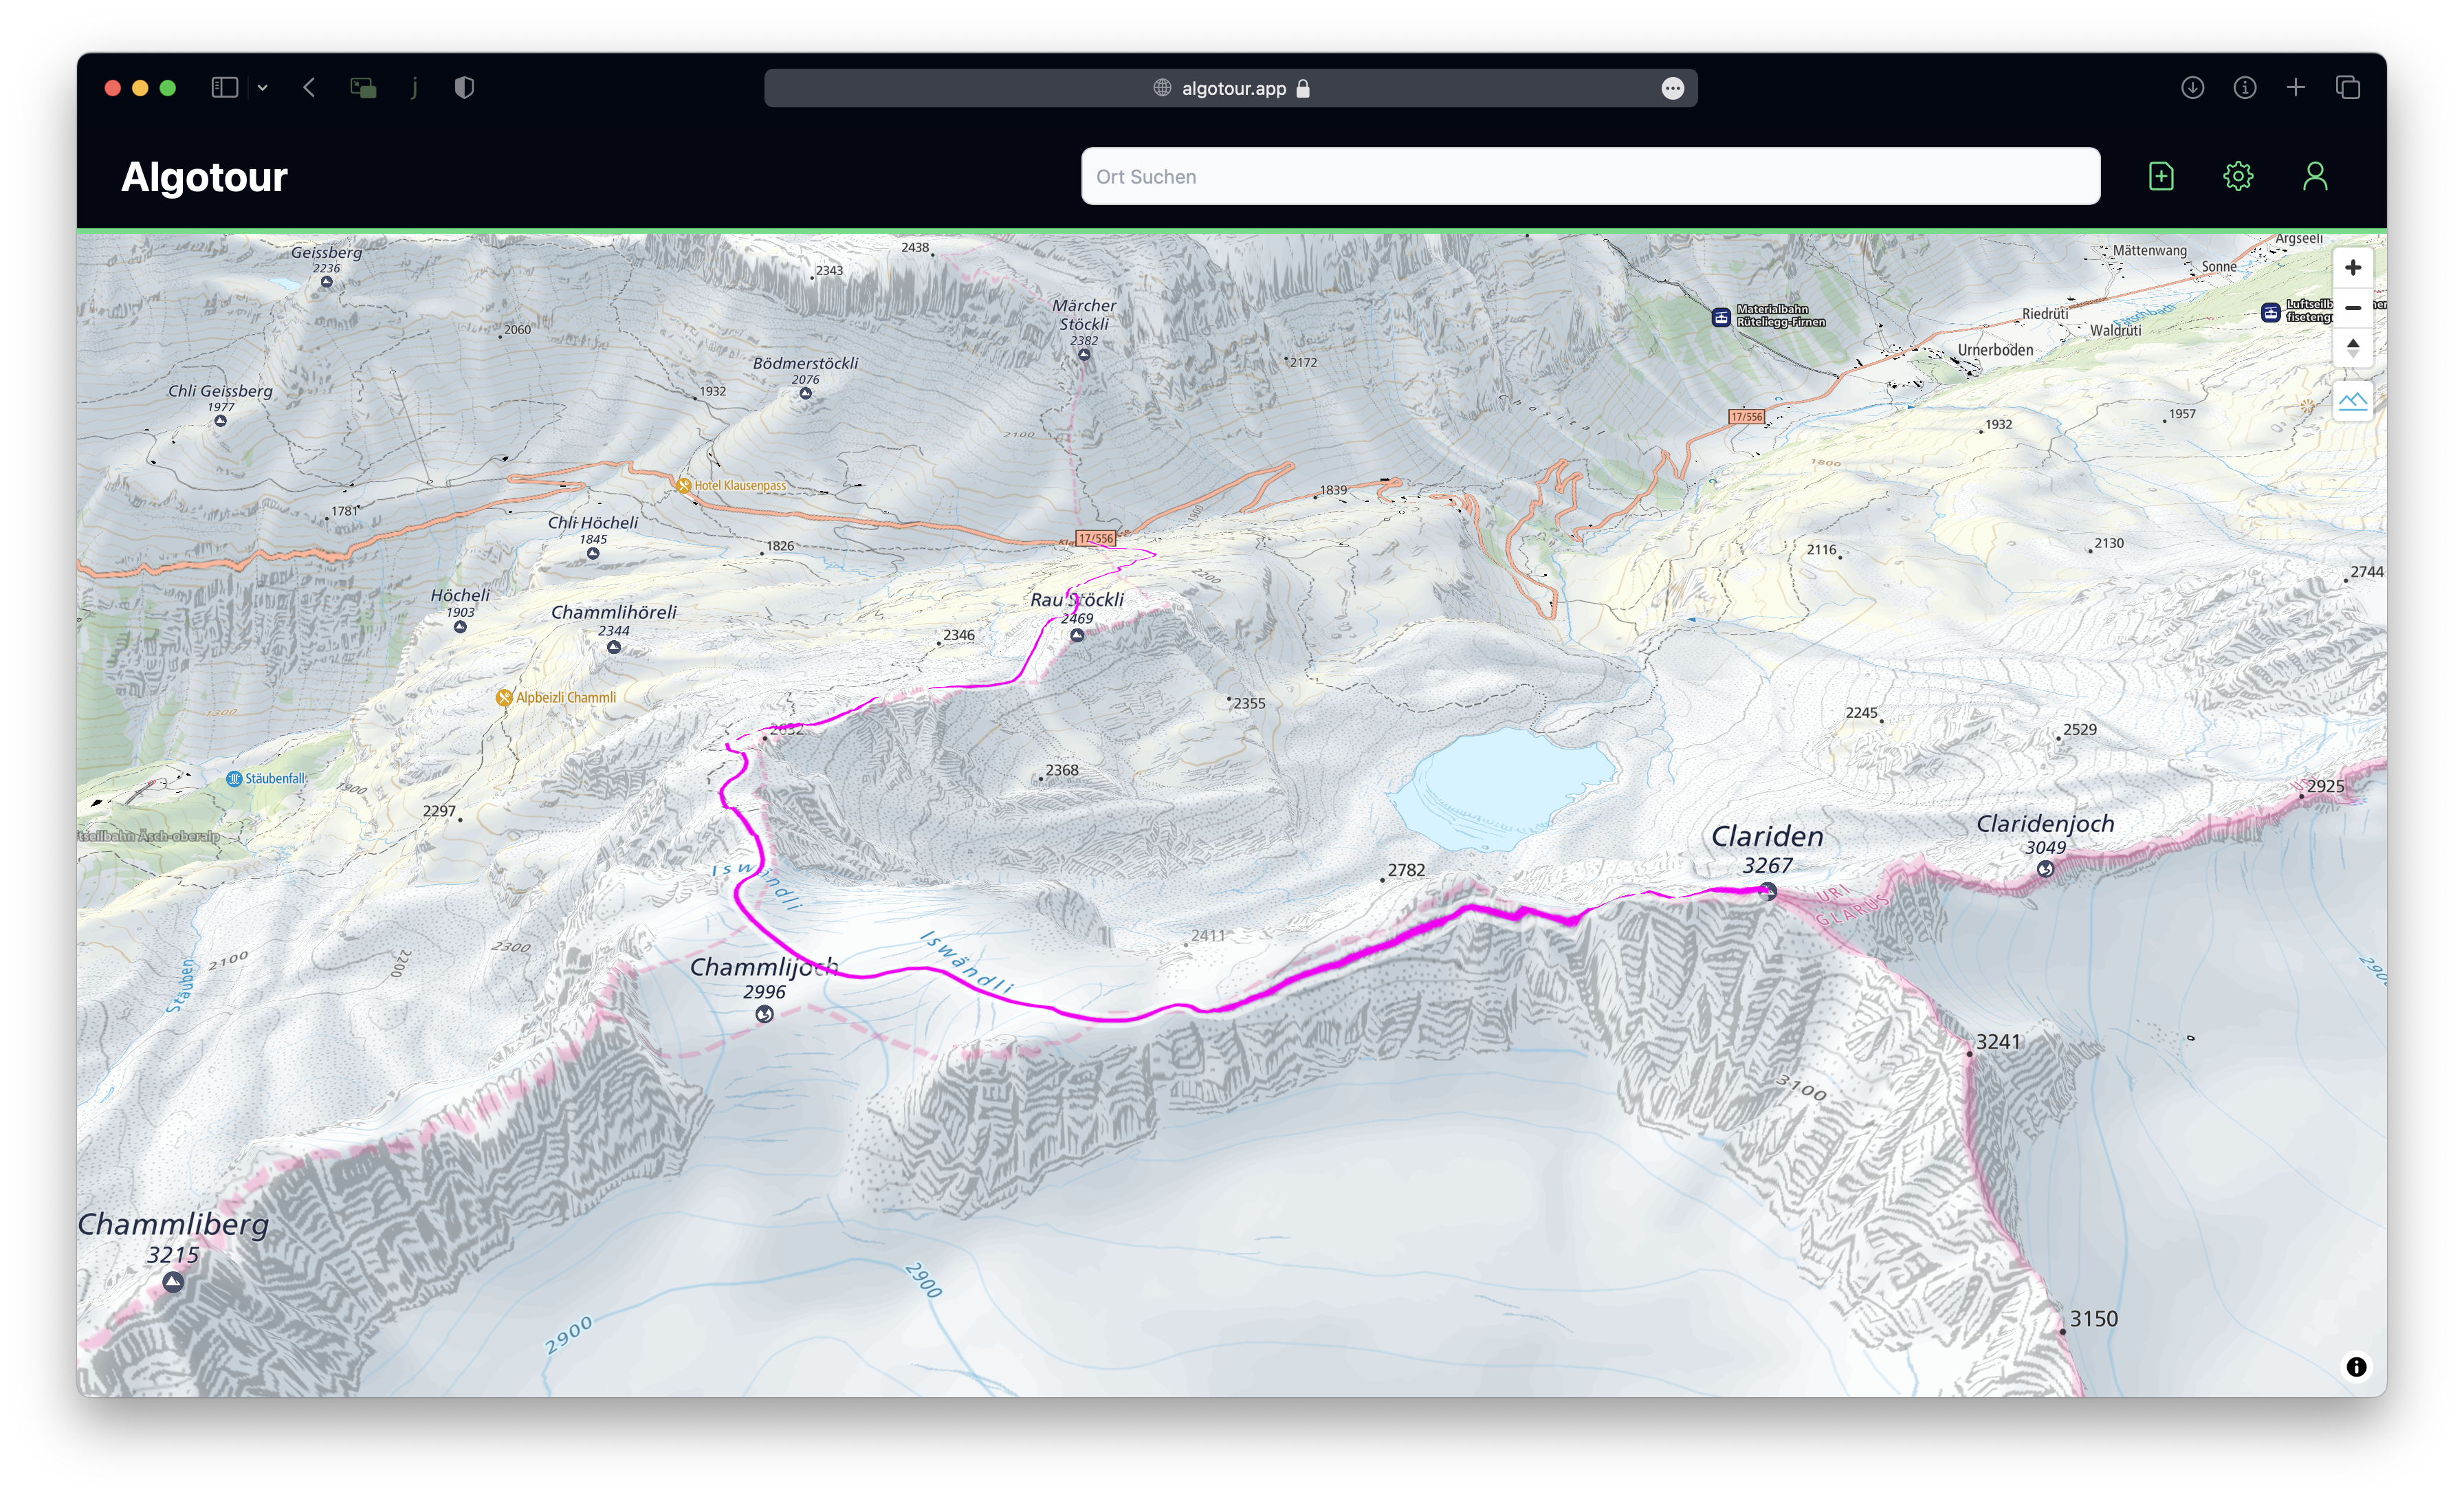
\includegraphics[width=\linewidth]{webapp}
    \caption{Nutzeroberfläche der Webapp, Tour auf den Clariden}\label{fig:mainui}
  \end{figure}
% \end{Mappage}

% \begin{multicols}{2}


% \end{multicols}
